El diagrama muestra un triángulo rectángulo y tres cuadrados.
El área del cuadrado más grande es 36 unidades$^2$, como se muestra en la figura \ref{fig:area13}.
\begin{figure}[H]
    \begin{center}
        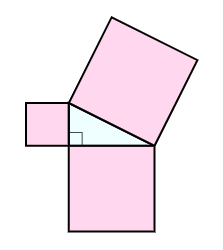
\includegraphics[width=0.4\textwidth]{../images/area13.png}
    \end{center}
    \caption{}
    \label{fig:area13}
\end{figure}

\begin{parts}
    \part \textbf{¿Cuáles pueden ser las áreas de los cuadrados más pequeños?}
    \begin{checkboxes}
        \choice 15 y 20
        \choice 6 y 30
        \choice 34 y 6
        \choice 10 y 16
        \choice 26 y 10
        \choice 24 y 12
        \choice 8 y 27
        \choice 6 y 6
    \end{checkboxes}
\end{parts}